As we mentioned in Section 2, decoders are used to perform inference of the error. After the decoder makes a guess of the channel error, the recovery operation can be implemented. However, increasing the accuracy of the decoder usually leads to higher computational complexity, making it slower at making guesses. The trade-off between accuracy and complexity is vital for quantum error correction. In Section 2, we discussed the details of MWPM. Here, we provide a review of a paper that confirms that adapting decoding algorithms to the specific noise characteristics of a quantum device creates more efficient and effective quantum error correction.

\subsection{Tensor-network decoder}

The biggest difference from MWPM is that MWPM only takes Pauli noise into account, and it assumes an uncorrelation between $X$ error and $Z$ error. But, the two-dimensional tensor-network method is provided with the noise map. It can be optimally adapted to arbitrary local noise, including non-Pauli noise, and can also handle correlated noise. The decoding algorithm involves constructing a square-lattice tensor network using information from the syndrome and the suspected noise map, then contracting the network using the time-evolving block decimation (TEBD) algorithm.

\subsubsection{Tensor Network States}

A tensor network can be visualized as a graph where each vertex represents a tensor, a multi-index array of complex numbers. The number of edges incident to a vertex corresponds to the number of tensor indices, with the dimension of an index called the bond dimension. When two vertices are connected by an edge, their corresponding indices are summed over (contracted), similar to matrix multiplication. A vertex can have incident edges not connected to another vertex, called physical indices, which are not contracted.

\subsubsection{Surface Code Wave Function}

The surface code wave function for any encoded state can be described as a projected entangled pair state (PEPS), represented on a square lattice where each tensor corresponds to a physical qubit, which is shown in Figure~\ref{fig:TN_layout}(a). The PEPS structure implies that the density operator can be expressed as a projected entangled pair operator (PEPO).
\subsubsection{Logical Channel Calculation}

For noiseless syndrome extraction, the logical channel $R_s \circ N$ can be calculated by computing all 16 elements of the Pauli transfer matrix: $C_{ij} = {\rm Tr}(L_i(R_s\circ N(L_j)))$
where $L_i$ , $L_j$ are logical Pauli operators, $N$ is noise map. The tensor-network structure preserves the PEPS form during the application of local noise $N$ , recovery  $R_s$, and logical Pauli $L_i$ , allowing  to be expressed as a multi-layer PEPS. Evaluating the trace involves tracing out pairs of physical indices, resulting in a tensor network with no physical indices. This tensor network can be compressed into a single layer by contracting along the time dimension. The resulting square-lattice tensor network can then be contracted using methods like treating the left-hand column as a matrix product state (MPS), evolving it by applying columns sequentially, and using singular value decomposition to control bond dimension growth. Alternatively, the square lattice tensor network can be contracted exactly by merging tensors in the left column into a single tensor, then contracting tensors from the remaining network column by column. The process is shown in the Figure~\ref{fig:TN_layout}.

\begin{figure}[h]
    \centering
    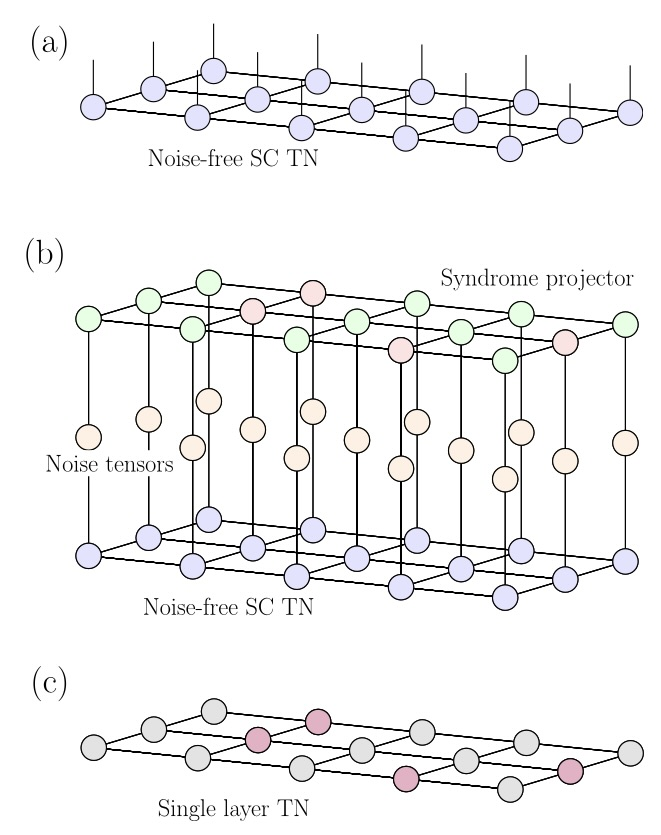
\includegraphics[width=0.4\textwidth]{sections/3_decoder/TN_layout.jpg}
    \caption{(a) A square-lattice PEPS depicting a surface code state, with each tensor having one physical index. (b) A tensor network representing an entry Cij of the Pauli transfer matrix of the logical channel for the surface code under a local noise map with noiseless syndrome extraction. There are three layers corresponding to the noiseless surface code state, local noise, and a syndrome projector, with physical indices traced out. (c) The same tensor network from (b) expressed as a single-layer tensor network which is obtained by vertically contracting the three layers.}
    \label{fig:TN_layout}
\end{figure}

\subsection{Recognizing critical noise parameters using simulation-based decoding}

The paper provides how to identify the most crucial noise in the noise map. If a surface code with a local physical noise map $N$. We can find the optimal decoder that achieves optimal performance for this noise map Then we adjust the miscalibrated decoder, with different parameter $N'$ . If one single noise parameter is different from the optimal parameter, but the result is identical to the optimal one, then we can indicate that the noise is not crucial. The paper have done some adaption about three primary noise features: coherence, inhomogeneity, and bias.
\subsubsection{Coherence}

Quantum noise involves systematic, non-random errors, such as unitary over-rotations due to imperfect gate control. Theoretical analyses of quantum error correcting codes often assume a Pauli noise model, where errors are characterized by random Pauli errors drawn from a probability distribution. This simplifies calculations, especially for stabilizer codes like the surface code, as Pauli noise can be efficiently simulated within the stabilizer formalism. However, physical systems rarely adhere exactly to this assumption. Non-Pauli noise types, such as amplitude damping and systematic over rotations due to imperfect gate control, are common but often overlooked. In order to differentiate from Pauli noise, the author refers to non-Pauli noise as coherent noise. Coherent noise introduces off-diagonal elements in the $\chi$ matrix representation of quantum channels, indicating interactions between different Pauli errors. Previous studies have shown that the surface code's performance can be significantly impacted by coherent noise, sometimes even more so than by Pauli noise. The paper investigates two noise models: single-qubit unitary rotations and systematic over-rotations in CNOT gates. The author compares the performance of different decoders, including an optimal decoder, a decoder considering only incoherent noise components (Pauli' decoder), and a standard minimum-weight perfect matching (MWPM) decoder applied separately to $X$ and $Z$ syndrome data. The paper reveals that adapting the decoder to consider the full noise map, including coherent components, can lead to performance improvements over decoders optimized solely for incoherent noise. However, the magnitude of this improvement is relatively small.

\subsubsection{Inhomogeneity}

Noise in many quantum computing system is spatially inhomogeneous, that is, it varies across different qubits in the device. The paper take noise model of amplitude-phase damping into account. As the \textbf{equation (6)(7)} shows, $\gamma$ represents damping probability and $\lambda$ scattering probabilities. We can assign it as relaxation time $T_1$ and the dephazing time $T_2$ by $e^{-t/T_2}$ = $\sqrt{(1-\gamma)(1-\lambda)}$ and $e^{-t/T_1} = 1 - \gamma$. In experiments, $T_1$ and $T_2$ times can vary significantly over different qubits in a device. The results of our simulations with different decoders are shown in Figure~\ref{fig:T1_fixed}. The first decoder is optimal, which is perfectly fit to the $T_1$ and $T_2$. The second 'uniform' one only have the average of $T_1$ and $T_2$ of each qubit. The third decoder 'ratio' only has information about ratio of $T_1$ and $T_2$ on each qubit. The fourth decoder is simply standard MWPM using a uniformly weighted syndrome graph. The result are clear that the optimal one which equipped with all the information about damping noise outperforms the standard one. The most interesting part is that even just have the ratio of $T_1$ and $T_2$ also improved significantly from the standard one.

\begin{figure}[h]
    \centering
    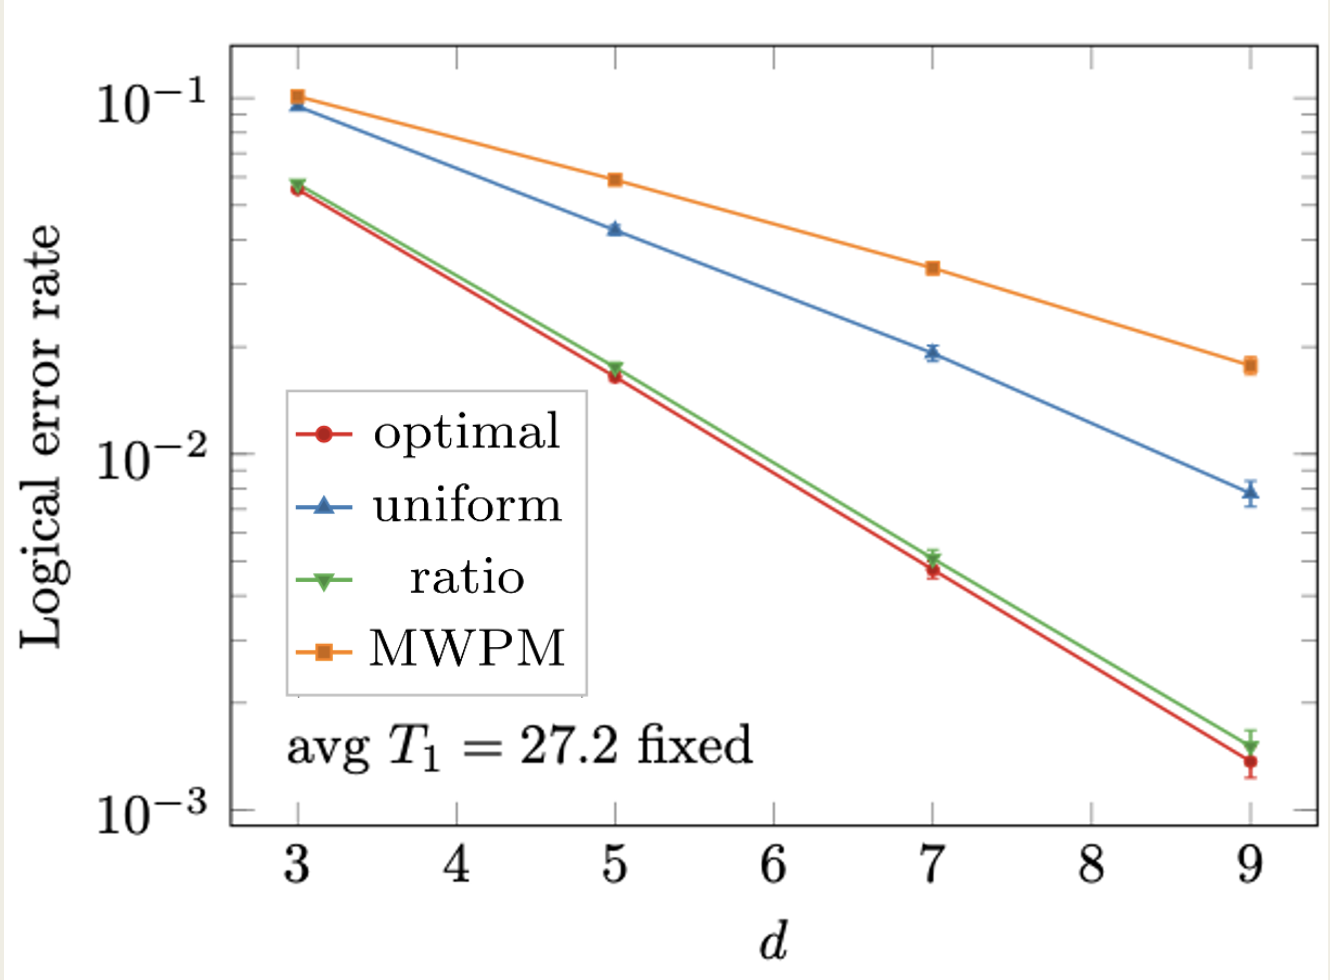
\includegraphics[width=0.4\textwidth]{sections/3_decoder/T1_fixed.png}
    \caption{}
    \label{fig:T1_fixed}
\end{figure}

$$ N_{APD}(\rho) =
    \left(\begin{array}{cc}
            \rho_{00} +  \gamma\rho_{11}          & \rho_{01}\sqrt{(1-\gamma)(1-\lambda)} \\
            \rho_{10}\sqrt{(1-\gamma)(1-\lambda)} & \rho_{11}(1-\gamma)
        \end{array}\right)
$$
$$=
    \left(\begin{array}{cc}
            1-\rho_{11}e^{-t/T_1} & \rho_{01}e^{-t/T_2} \\
            \rho_{01}^*e^{-t/T_2} & \rho_{11}e^{-t/T_1}
        \end{array}\right)
$$


\subsection{Bias}

The paper defines a Pauli noise model as biased when one Pauli error occurs with significantly higher probability than others. As the paragraph aforementioned, we designate either $X$, $Y$, or $Z$ as the dominant error, and the surface code's performance heavily relies on the local basis used for defining checks. The author focus is on single-qubit $Y$-biased Pauli noise, where $p_X$ = $p_Z$ , $p := p_X +p_Y +p_Z$, and $\eta := \frac{p_Y}{p_X + p_Z}$ . The simulation results, depicted in Figure~\ref{fig:eta}, illustrate the effects of depolarizing (unbiased) noise corresponding to $\eta$ = 0.5 and biased noise with $\eta$ = 100. For depolarizing noise, as shown in Figure~\ref{fig:eta}(a), the miscalibrated decoder achieves nearly same logical error rates compared to the optimal decoder, with the threshold barely altering. On the other hand, under biased noise with fixed $\eta = 100$, as shown in Figure~\ref{fig:eta}(b), there is a significant difference observed between the two decoders. The logical error rate for the largest system size with the miscalibrated decoder. These findings suggest that sensitivity to decoder miscalibration escalates with noise bias. Notably, the decoder needs a number of information about the bias $\eta$ to perform optimally
\begin{figure}[h]
    \centering
    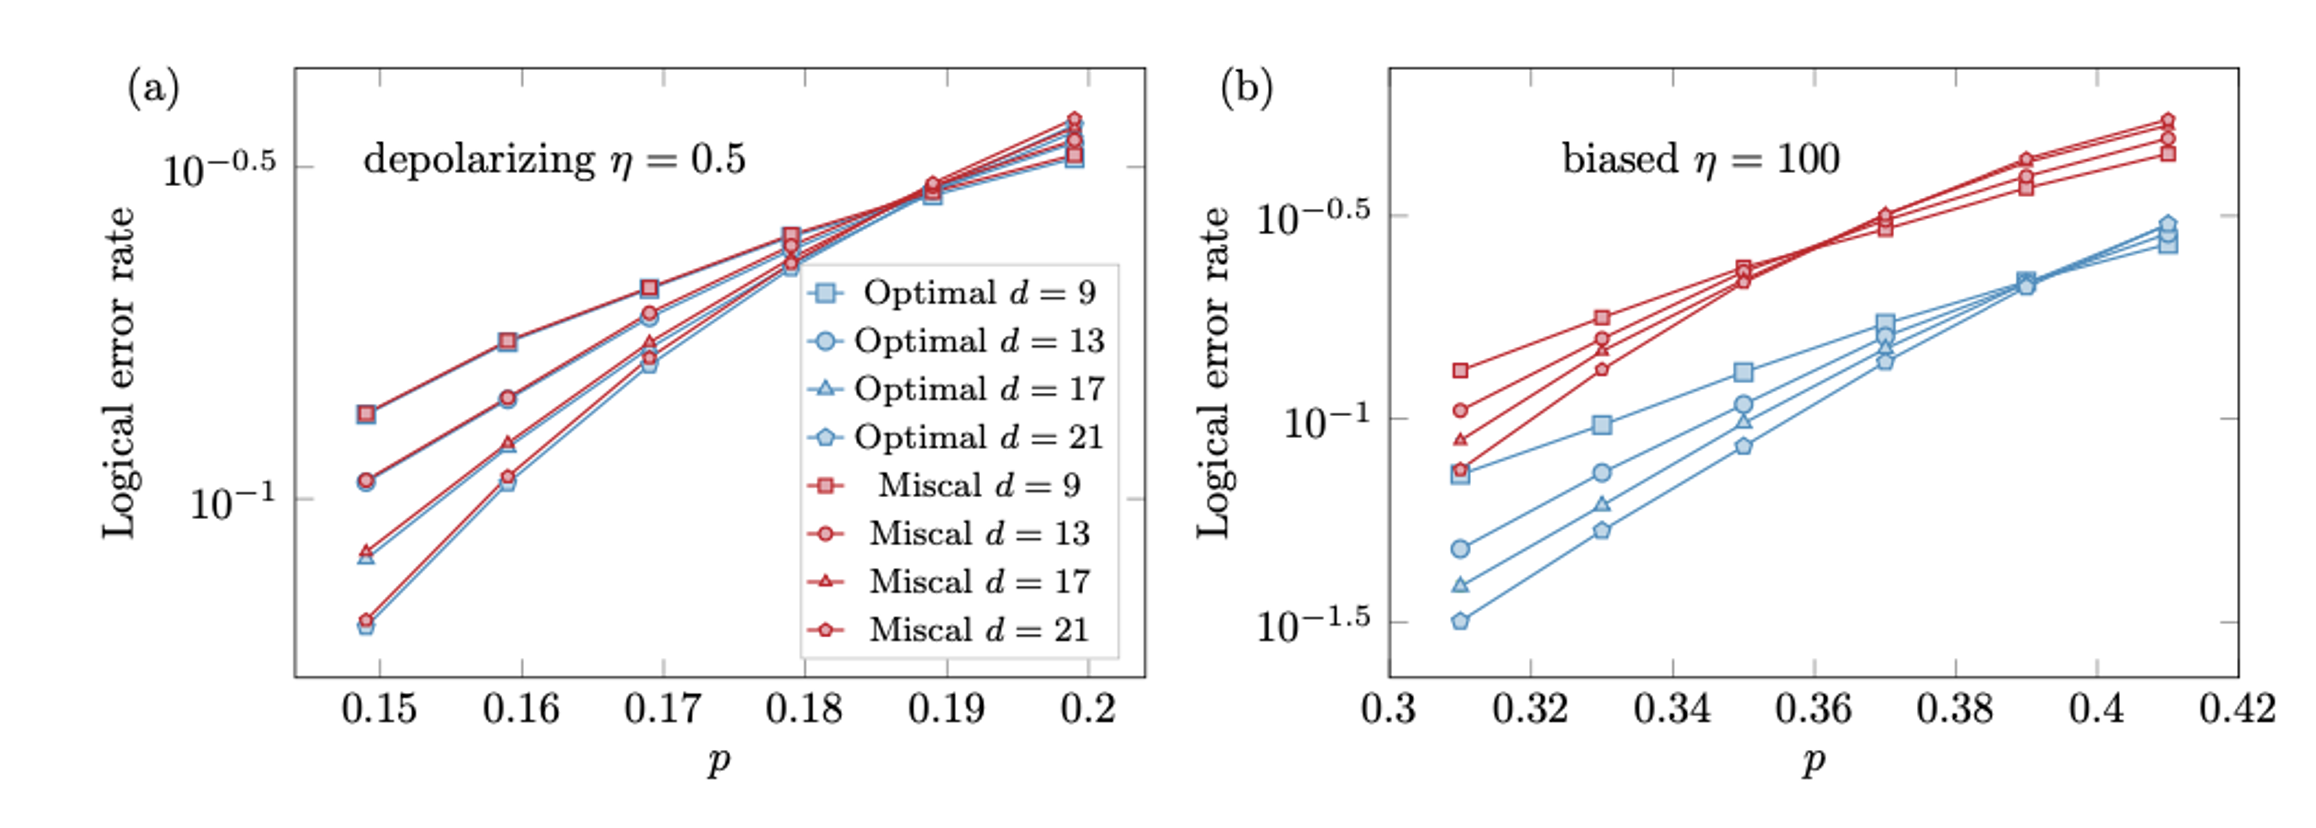
\includegraphics[width=0.5\textwidth]{sections/3_decoder/eta.png}
    \caption{The effect of noise bias on surface-code decoding. 'Optimal' means that the noise model input to the decoder is exactly the physical noise model, and 'Miscal' means that the average infidelity in the decoder noise model is mischaracterized pdec = p/2. (a) physical noise model is depolarizing noise, while in (b) it is biased noise with $\eta$ = 100}
    \label{fig:eta}
\end{figure}

By focusing on coherence, inhomogeneity, and bias, and understanding their impact on decoder performance, the paper provides a framework for optimizing surface-code decoders by leveraging detailed noise information. This targeted approach not only aids in developing better decoders but also informs the design of noise characterization techniques, ensuring that future quantum computing systems can maintain high levels of fault tolerance with reduced overhead.